% This file was created with tikzplotlib v0.10.1.
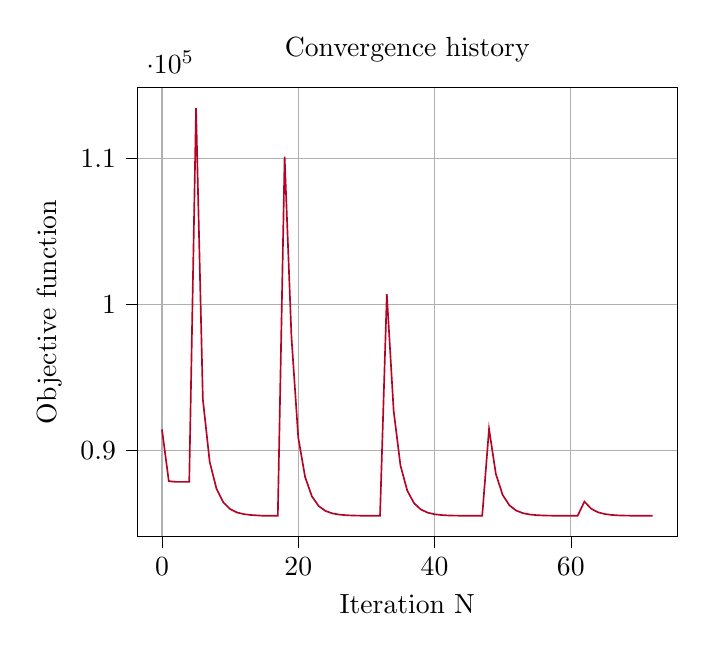
\begin{tikzpicture}

\definecolor{darkgray176}{RGB}{176,176,176}
\definecolor{firebrick180438}{RGB}{180,4,38}

\begin{axis}[
tick align=outside,
tick pos=left,
title={Convergence history},
x grid style={darkgray176},
xlabel={Iteration N},
xmajorgrids,
xmin=-3.6, xmax=75.6,
xtick style={color=black},
y grid style={darkgray176},
ylabel={Objective function},
ymajorgrids,
ymin=84140.4973908178, ymax=114805.744111147,
ytick style={color=black}
]
\addplot [semithick, firebrick180438]
table {%
0 91442.5585116738
1 87907.0802673692
2 87857.9447685309
3 87857.9100270034
4 87857.9100269807
5 113411.869260223
6 93505.0018496608
7 89235.3746151231
8 87381.5440623512
9 86457.9648560041
10 85996.1760131869
11 85765.281682217
12 85649.8296002172
13 85592.1081534132
14 85563.2480255216
15 85534.3722417418
16 85534.3878951324
17 85534.3878951312
18 110096.797133131
19 97799.8759770601
20 90891.7212739527
21 88198.9505290925
22 86866.6612601459
23 86200.5244558835
24 85867.4560524951
25 85700.9217962858
26 85617.6482232326
27 85576.0166650051
28 85555.2021154657
29 85544.7949279598
30 85534.3909379801
31 85534.3878951313
32 85534.3878951312
33 100699.072907405
34 92723.1360264712
35 88977.1200459707
36 87255.1478385516
37 86394.7673237219
38 85964.5769678377
39 85749.4821664708
40 85641.9346284159
41 85588.1612506259
42 85561.2746048028
43 85547.8312536361
44 85541.1095923607
45 85534.3887969695
46 85534.3878951312
47 85534.3878951311
48 91483.9254634474
49 88395.0236672997
50 86959.7414970811
51 86247.0639374188
52 85890.7258299826
53 85712.5566607045
54 85623.4679272938
55 85578.9272853879
56 85556.6576042204
57 85545.522770877
58 85539.9550574051
59 85534.3884677326
60 85534.3878951312
61 85534.3878951311
62 86505.1326155232
63 86016.1566215303
64 85775.2677758983
65 85654.827121016
66 85594.6073942911
67 85564.4976739601
68 85549.4428034945
69 85541.9153805318
70 85534.3891781949
71 85534.3878951312
72 85534.3878951311
};
\end{axis}

\end{tikzpicture}
